\documentclass[11pt]{beamer}
\usepackage{../settings}

\title{DISTRIBUTION SHIFT}
\subtitle{A Study on Their Effects on Statistical Models and Strategies for Mitigation}
\date{}
\author{Andrea Spinelli, Giacomo Amerio,\\Giovanni Lucarelli, Tommaso Piscitelli}
\institute{University of Trieste}
\titlegraphic{\hfill
\includegraphics[height=1.5cm]{assets/logo100_orizzontale.pdf}}

\begin{document}

\section{Introduction}

\begin{frame}{Dataset shift}
\begin{itemize}
    \item \textbf{Dataset shift} is a common problem in machine learning.
    
    \item It occurs when the distribution of the training data differs from the distribution of the test data.
   
    \item This can lead to a decrease in the performance of the model.
\end{itemize}    
    The two most common and well-studied causes of dataset shift are:
    \begin{itemize}
    	\item Sample selection bias
    	
    	\item non stationary environments
    \end{itemize}

\end{frame}

\begin{frame}{Aims of project}

\vspace{0.8cm}
This project aims to evaluate the impact of simple  \textbf{Covariate shift} in the input distribution on the performance of robust models within the context of a synthetic binary classification task.

Key questions addressed in this study include:
\begin{itemize}
	\item How do different types of covariate shifts affect the performance of robust models?
	\item Are certain models inherently more robust to simple covariate shifts?
	\item What strategies can be employed to improve model performance following such shifts?
\end{itemize}
\end{frame}

\begin{frame}{Covariate shift}
Can be formally defined as follows. Consider an input variable \( X \) and a response variable \( Y \), where \( X \to Y \) represents the relationship between the two. Let \( P_{\text{tra}} \) denote the probability distribution of the training data and \( P_{\text{tst}} \) denote the probability distribution of the test data. A covariate shift occurs when:  
\[
P_{\text{tra}}(Y \mid X) = P_{\text{tst}}(Y \mid X) \quad \text{but} \quad P_{\text{tra}}(X) \neq P_{\text{tst}}(X)\,.
\]
\begin{figure}[H]
	\centering
	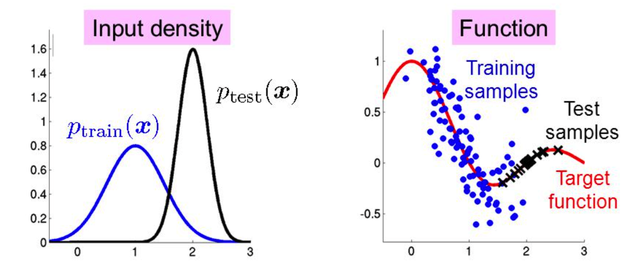
\includegraphics[width=0.8\textwidth]{../assets/immagine.png} 
    \label{fig:covariate-shift}
\end{figure}
\end{frame}

\begin{frame}{Example}
Consider a model designed to distinguish between cats and dogs:

\vspace{0.5cm}
\begin{minipage}[t]{0.45\textwidth} % 45% della larghezza per l'immagine
  \begin{flushleft}
	\textbf{\textcolor{blue}{Training set:}}
  \end{flushleft}
\centering
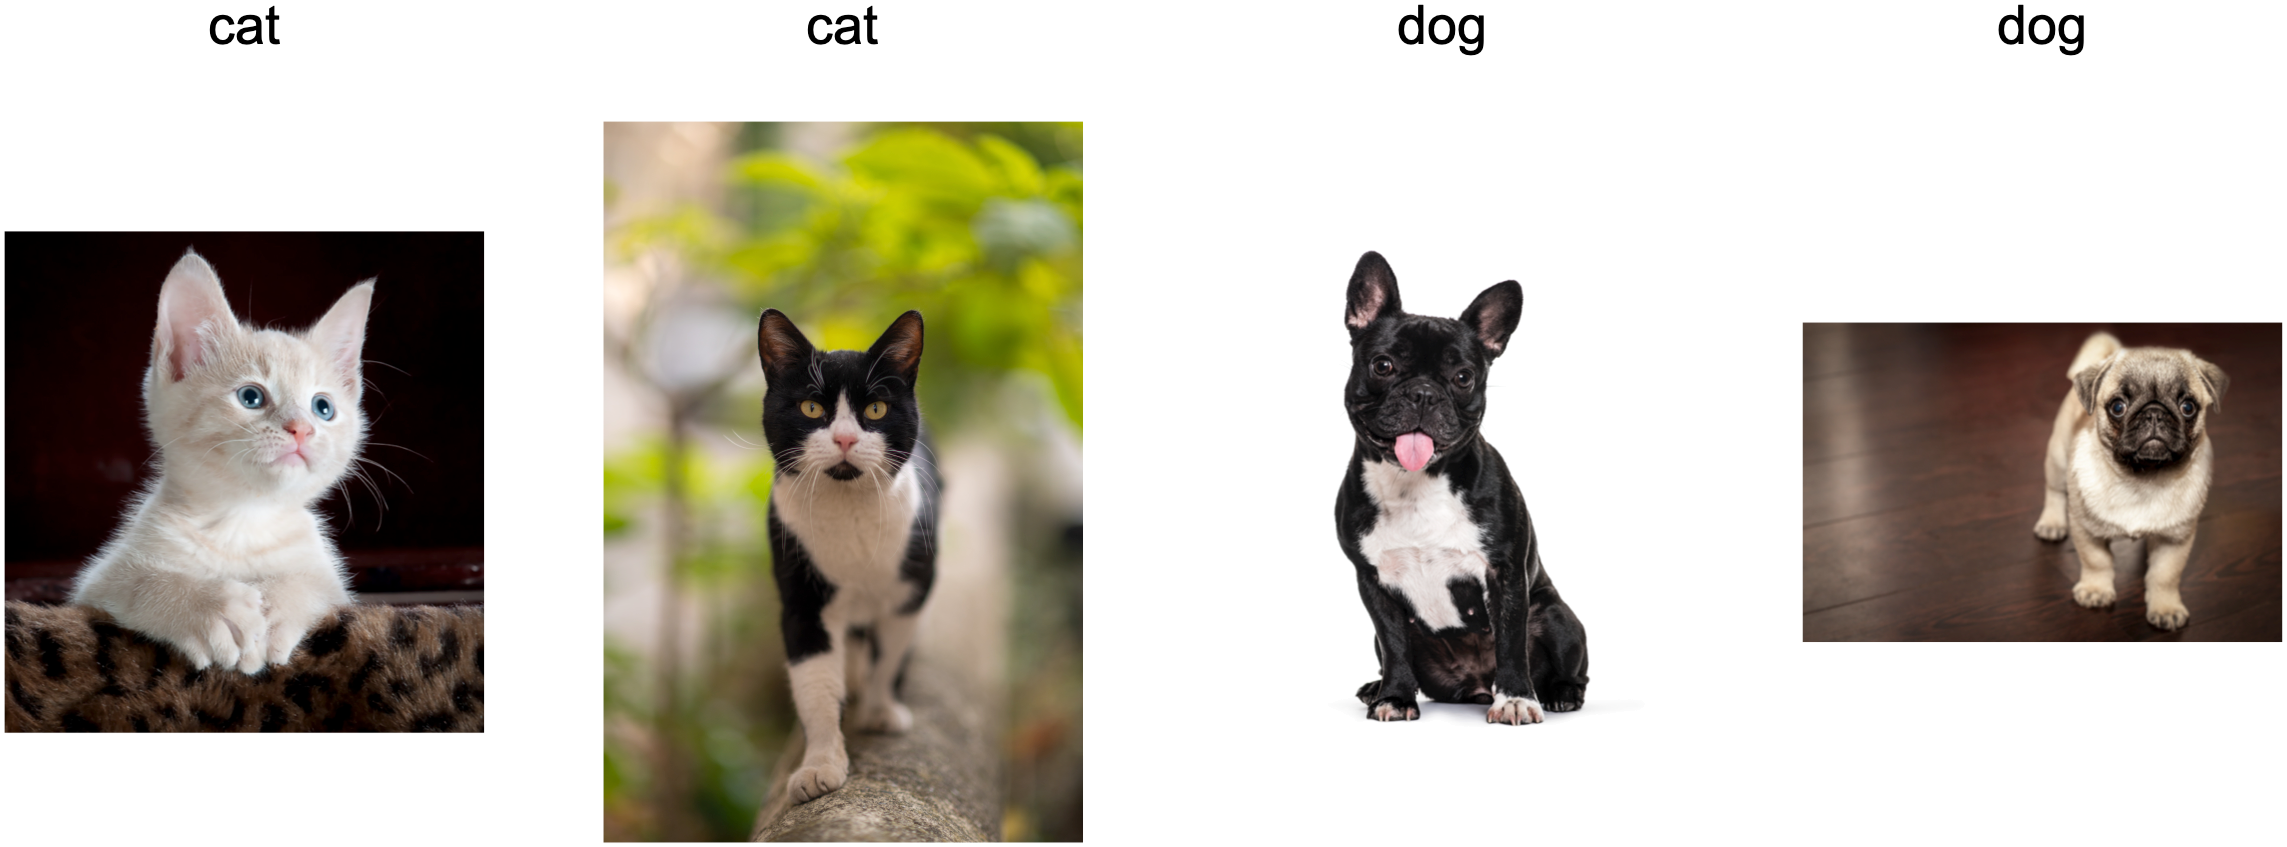
\includegraphics[width=5cm]{../assets/cat-dog-train.png}
\label{fig:cani-gatti}
\vspace{-0.5cm}
\begin{flushleft}
	\textbf{\textcolor{blue}{Test set:}}
\end{flushleft}
\centering

\includegraphics[width=5cm]{../assets/cat-dog-test.png}
\label{fig:cani-gatti}

\end{minipage}
\hfill
\begin{minipage}[t]{0.45\textwidth} % 45% della larghezza per la didascalia
\begin{itemize}
	\item Model will not accurately distinguish between cats and dogs because the feature distribution will differ.
	\item Changes in the input distribution can significantly impact the model's accuracy.
\end{itemize}
\end{minipage}
	
\end{frame}


\begin{frame}{Inaccurate model}
\begin{figure}[H]
	\centering
	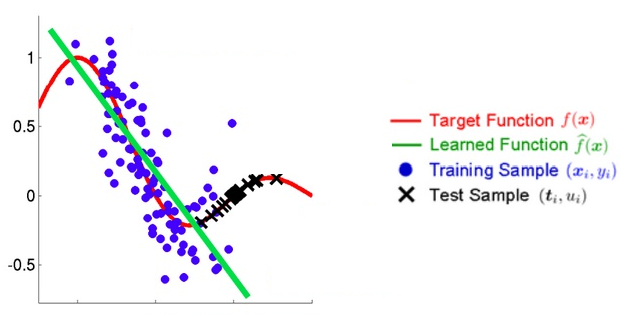
\includegraphics[width=0.7\textwidth]{../assets/covariate_shift.png} 
	\caption{Example of inaccurate model.}
	%\label{fig:inaccurate-model}
\end{figure}
In this study, we analyze the effects of distribution shift on different statistical models and propose strategies for its mitigation.
\end{frame}

\end{document}